% Created 2024-02-09 Fri 16:19
% Intended LaTeX compiler: pdflatex
\documentclass[11pt]{article}
\usepackage[utf8]{inputenc}
\usepackage[T1]{fontenc}
\usepackage{graphicx}
\usepackage{grffile}
\usepackage{longtable}
\usepackage{wrapfig}
\usepackage{rotating}
\usepackage[normalem]{ulem}
\usepackage{amsmath}
\usepackage{textcomp}
\usepackage{amssymb}
\usepackage{capt-of}
\usepackage{hyperref}
\usepackage{minted}
\usepackage[a4paper,margin=20mm]{geometry}
\usepackage{amsmath}
\usepackage{amsfonts}
\usepackage{stmaryrd}
\usepackage{bm}
\usepackage{minted}
\usemintedstyle{emacs}
\usepackage[T1]{fontenc}
\usepackage[scaled]{beraserif}
\usepackage[scaled]{berasans}
\usepackage[scaled]{beramono}
\newcommand{\tr}{\textsf{T}}
\newcommand{\grad}{\bm{\nabla}}
\newcommand{\av}[2][]{\mathbb{E}_{#1\!}\left[ #2 \right]}
\newcommand{\Prob}[2][]{\mathbb{P}_{#1\!}\left[ #2 \right]}
\newcommand{\logg}[1]{\log\!\left( #1 \right)}
\newcommand{\pred}[1]{\left\llbracket { \small #1} \right\rrbracket}
\newcommand{\e}[1]{{\rm e}^{#1}}
\newcommand{\dd}{\mathrm{d}}
\DeclareMathAlphabet{\mat}{OT1}{cmss}{bx}{n}
\newcommand{\normal}[2]{\mathcal{N}\!\left(#1 \big| #2 \right)}
\newcounter{eqCounter}
\setcounter{eqCounter}{0}
\newcommand{\explanation}{\setcounter{eqCounter}{0}\renewcommand{\labelenumi}{(\arabic{enumi})}}
\newcommand{\eq}[1][=]{\stepcounter{eqCounter}\stackrel{\text{\tiny(\arabic{eqCounter})}}{#1}}
\newcommand{\argmax}{\mathop{\mathrm{argmax}}}
\newcommand{\Dist}[2][Binom]{\mathrm{#1}\left( \strut {#2} \right)}
\author{Adam Prügel-Bennett}
\date{\today}
\title{Advanced Machine Learning Subsidary Notes\\\medskip
\large Lecture 24: Generative Models}
\hypersetup{
 pdfauthor={Adam Prügel-Bennett},
 pdftitle={Advanced Machine Learning Subsidary Notes},
 pdfkeywords={},
 pdfsubject={},
 pdfcreator={Emacs 27.1 (Org mode 9.3)}, 
 pdflang={English}}
\begin{document}

\maketitle

\section{Keywords}
\label{sec:org5308e08}
\begin{itemize}
\item Conditional Independence, Graphical models, LDA
\end{itemize}

\section{Main Points}
\label{sec:orge6c945d}


\subsection{Overview}
\label{sec:orge8b3eb8}
\begin{itemize}
\item We have so far considered building rather simple probabilistic models
\item But what if we want to do inference on a more complicated
problem, e.g.
\begin{itemize}
\item We might want to write a fault diagnosis system for a car
\item Or we want to create an AI doctor
\item The model of the spread of a virus
\end{itemize}
\item Here we have a vast number of random variables with complicated
relationships between them
\item To help design our system we can build a \emph{graphical model}
showing the causal relationships between random variables
\end{itemize}

\subsection{Conditional Independence}
\label{sec:orgeb8730f}
\begin{itemize}
\item \textbf{Independence}
\begin{itemize}
\item Two random variable \(X\) and \(Y\) are independent if
\begin{align*}
\Prob{X,Y} = \Prob{X}\,\Prob{Y}
\end{align*}
\item Independence can significantly speed up calculations, e.g.
\begin{align*}
\av{X^2\,Y} = \sum_{X,Y} X^2\,Y\,\Prob{X,Y} 
= \left( \sum_{X} X^{2} \, \Prob{X} \right)\, \left( \sum_{Y} Y \Prob{Y} \right)
\end{align*}
\begin{itemize}
\item If \(X\) and \(Y\) takes \(n\) and \(m\) values then without
independence the double sum \(\sum_{X,Y}\) would be over
\(n\times m\) possible values
\item With independence we can compute these sums independently so
it just takes \(m+n\)  additions
\end{itemize}
\item When we have large systems with many independent variables
then the time saving is often the difference between
calculations being feasible or infeasible
\item Unfortunately in most complex systems there is likely to be
some dependence between random variables
\end{itemize}
\item \textbf{Conditional Independence}
\begin{itemize}
\item A weaker notion than full independence is \emph{conditional independence}
\item We say that \(X\) and \(Y\) are conditionally independent given
\(Z\) if
$$ \Prob{X,Y|Z} = \Prob{X|Z}\,\Prob{Y|Z} $$
\item Again this can lead to significant speed up in evaluating
expectations, e.g.
\begin{align*}
\av{X^{2}\,Y\,Z^{3}} &= \sum_{X,Y,Z} \Prob{X,Y,Z} X^{2}\,Y\,Z^{3}
= \sum_{X,Y,Z} \Prob{X,Y|Z}\,\Prob{Z} X^{2}\,Y\,Z^{3} \\
&= \sum_{Z} Z^{3} \left( \sum_{X} X^{2}\,\Prob{X|Z}\right)
\left( \sum_{Y} Y\, \Prob{Y|Z}\right)
\end{align*}
\begin{itemize}
\item If \(X\), \(Y\) and \(Z\) have \(l\), \(m\) and \(n\) values respectively, then,
ignoring conditional independence, this expectation would
require \(l\times m\times n\) additions; using conditional
independence it only requires \(n\times(l+m)\) additions
\end{itemize}
\item Although conditional dependence doesn't imply causality,
if random variables \(X\) and \(Y\) are not directly causally
related they will be conditionally independent
\item This is important prior information we can build into our
model
\end{itemize}
\end{itemize}

\subsection{Graphical Models}
\label{sec:org2524c1a}
\begin{itemize}
\item In graphical models we represent each random variable as a node
in a graph
\item There are two main classes of graphical models
\begin{itemize}
\item Bayesian Belief Networks
\begin{itemize}
\item use directed graphs
\item we will spend most of our time discussing these
\end{itemize}
\item Markov Fields
\begin{itemize}
\item uses adirected graphs
\item these are used in graphics a lot
\item won't really discuss these
\end{itemize}
\end{itemize}
\item Each causal connection we represent as a directed edge in a
Bayesian Belief Network
\begin{itemize}
\item if \(A\) directly influences \(B\) we represent this as
\begin{center}

\includegraphics[width=0.17\textwidth]{figures/atob.pdf}
\end{center}
\end{itemize}
\item \textbf{Cakes}
\begin{itemize}
\item We consider the following example
\item Abi and Ben both bake cakes and like to bring them into the
coffee room
\item They do this randomly without consulting with each other
\item Abi will bring in cakes 20\% of the time: \(\Prob{A=1} = 0.2\)
\item Ben will bring in cakes 10\% of the time: \(\Prob{B=1} = 0.1\)
\item 90\% of the time if either Abi or Ben have put cakes in the
coffee room there is some left when I enter
\(\Prob{C=1|A=1,B=0} = \Prob{C=1|A=0,B=1}=0.9\)
\item If they both make cake then there is always cake left  \(\Prob{C=1|A=1,B=1}=1\)
\item If neither Abi or Ben has made cake there is still a 5\%
chance someone else has put cake in the coffee room \(\Prob{C=1|A=0,B=0}=0.05\)
\item We note that \(\Prob{C=0|A,B}=1-\Prob{C=1|A,B}\) as
\(\sum_{C\in\{0,1\}}\Prob{C|A,B}=1\)
\item We can draw the causal relationships as
\begin{center}

\includegraphics[width=0.3\textwidth]{figures/acb.pdf}
\end{center}
\item This allows us to break down the joint probability as
\begin{align*}
\Prob{A,B,C} &\eq \Prob{C,B|A}\,\Prob{A} \\
&\eq \Prob{C|A,B}\,\Prob{B|A}\,\Prob{A} \eq \Prob{C|A,B}\,\Prob{B}\,\Prob{A}
\end{align*}
\explanation
\begin{enumerate}
\item Using the definition of conditional probability (this is always true)
\item Using the definition of conditional probability again (this is always true)
\item Using the fact that \(B\) and \(A\) are independent (there
is no arrow between them in the graphical
representation) so \(\Prob{B|A}=\Prob{B}\)
\begin{itemize}
\item From the graphical representation we can immediately write
down a simple form for this joint distribution
\end{itemize}
\end{enumerate}
\item We can use this decomposition to help us compute various probabilities
\item (To compute probabilities we use the fact that the
expectation of an indicator function \(\pred{\text{predicate}}\) is
equal to the probability \(\Prob{\text{predicate}}=\av{\,\pred{\text{predicate}}}\)
\begin{itemize}
\item The indicator function \(\pred{\text{predicate}}\) equals 1
if the predicate is true and 0 otherwise)
\end{itemize}
\item Let's compute the probability there are cakes
$$ \Prob{C=1} = \sum_{A,B,C\in\{0,1\}}
       \pred{C=1} \Prob{A,B,C} = \sum_{A,B\in\{0,1\}}
       \Prob{C=1|A,B} \Prob{A}\,\Prob{B} = 0.303 $$
\begin{itemize}
\item See Section \ref{sec:exCakes} for details of the calculation
(this is an exercise that should really help)
\item Here we exhaustively sum over all variables
\end{itemize}
\item Let us consider what happens when we observe a random variable
\begin{itemize}
\item In graphical models we often shade observed random variables
\end{itemize}
\begin{center}

\includegraphics[width=0.3\textwidth]{figures/acob.pdf}
\end{center}
\begin{itemize}
\item Let's compute quantities conditioned on an observation of \(C\)
$$ \Prob{A,B|C} =\frac{\Prob{A,B,C}}{\Prob{C}} $$
\item Thus \(\Prob{A,B|C=1} = \Prob{A,B,C=1}/\Prob{C=1}\)
\item Using this we can compute
\begin{align*}
\Prob{A=1,B=1|C=1} &= 0.066, &
\Prob{A=1|C=1} &=0.630, &
\Prob{B=1|C=1} &= 0.317
 \end{align*}
\item We note that \(\Prob{A=1,B=1|C=1} \neq \Prob{A=1|C=1} \, \Prob{B=1|C=1}\)
\item That is once we observe \(C\) then \(A\) and \(B\) are no
longer independent
\end{itemize}
\item We can extend our model further
\begin{itemize}
\item We suppose that Dave likes cakes so if there is a cake in
the coffee room there is a 80\% chance that I will see
him eating a cake: \(\Prob{D=1|C=1}=0.8\)
\item Even if there are no cakes in the coffee room there is a
10\% chance that Dave has bought his own cake: \(\Prob{D=1|C=0}=0.1\)
\item Eli also likes cakes: there is a 60\% chance that I will
see her eating cakes if there are cakes in the coffee
room: \(\Prob{E=1|C=1}=0.6\)
\item But she never buys herself cakes \(\Prob{E=1|C=0}=0\)
\item We can depict the dependencies of the this large model
\begin{center}
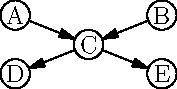
\includegraphics[width=0.3\textwidth]{figures/abcde_g.pdf}
\end{center}
\begin{align*}
\Prob{A,B,C,D,E} &= \Prob{C,D,E|A,B}\,\Prob{B}\,\Prob{A} \\
&= \Prob{D|C}\,\Prob{E|C}\, \Prob{C|A,B}\,\Prob{B}\,\Prob{A}
\end{align*}
\begin{itemize}
\item where we have used the conditional independence
\item note that \(D\) and \(E\) are conditionally independent of \(A\)
and \(B\) given \(C\)
\item That is, these probabilities will depend on events \(A\) and
\(B\), but once I know there are cakes in the coffee room it
doesn't matter who put them there
\item We can compute probabilities for this larger system
\begin{align*}
\Prob{D=1} &= 0.3121, & \Prob{E=1} &= 0.1818, &
\Prob{D=1,E=1} &= 0.14544
\end{align*}
so \(\Prob{D,E}\neq\Prob{D}\,\Prob{E}\)
\item \(D\) and \(E\) are not independent variables as they coupled
through \(C\)
\item However when we observe \(C\)
   \begin{center}
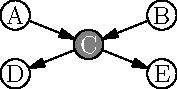
\includegraphics[width=0.3\textwidth]{figures/code.pdf}
\end{center}
then \(\Prob{D,E|C}\eq\Prob{D|C}\,\Prob{E|C}\)
\begin{itemize}
\item E.g.
\end{itemize}
\begin{align*}
\Prob{D=1|C=1} &= 0.8 & \Prob{E=1|C=1} &= 0.6 &
\Prob{D=1,E=1|C=1} &= 0.48
\end{align*}
\end{itemize}
\end{itemize}
\end{itemize}
\end{itemize}

\subsection{Latent Dirichlet Allocation}
\label{sec:orga2ae2c3}
\begin{itemize}
\item Most probabilistic models can be represented as a graphical model
\item There are times when this isn't particularly useful
\item But it can just help us to understand what is going on
\item We consider an example of this  called \textbf{Latent Dirichlet Allocation}
\begin{itemize}
\item This is sometimes known as LDA, but should not be confused with
\emph{linear discriminant analysis}
\end{itemize}
\item LDA is used to model topics in a set of documents (or \emph{corpus})
\item We want to identify a set of topics
\item The topics are associated with particular words
\item The documents will be associated with a small number of topics
\item To model this we build a \emph{generative model}
\begin{itemize}
\item This is natural to build
\item Although it seems the wrong way around---we don't want to
build a corpus of documents
\item But Bayes's rule allows us to invert this
\end{itemize}
\item Let us start with some definitions
\begin{itemize}
\item We consider generating a corpus of documents
$$ \mathcal{C} = \{d_i | i = 1,\, 2,\, \ldots |\mathcal{C}|\} $$
\item Each document consists of a set of words
$$ d = \left(w_1^{(d)},\, w_2^{(d)},\, \ldots,\,
       w_{N_d}^{(d)}\right) $$
\item We assume there is a set of topics
$$ \mathcal{T}=\{t_1,\,t_2,\,\ldots,\, t_{|\mathcal{T}|}\} $$
\item We associate a probability, \(\theta^{(d)}_t\), that a word in
document \(d\) relates to a topic \(t\)
\begin{center}
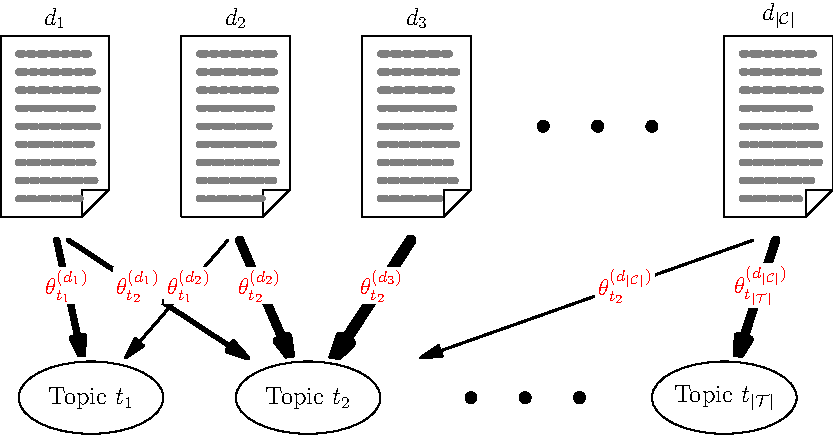
\includegraphics[width=0.6\textwidth]{figures/topicModelWtoT.pdf}
\end{center}
\item We associate a probability \(\phi^{(t)}_w\) that a word, \(w\), is
related to a topic \(t\)
\begin{center}
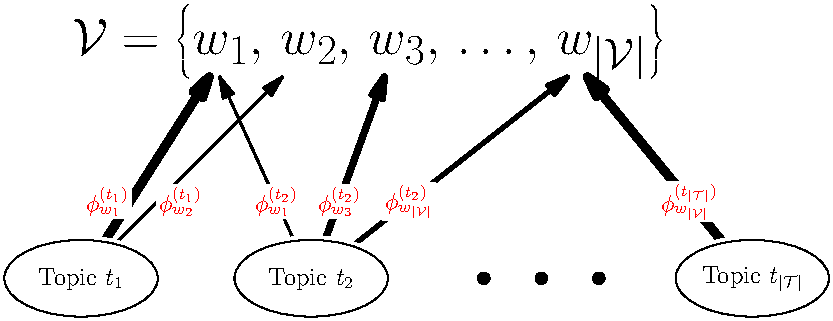
\includegraphics[width=0.6\textwidth]{figures/topicModel.pdf}
\end{center}
\item Most documents are predominantly about a few topics and most
topic have a small number of words associated to them
\item We can generate probability vectors \(\bm{\theta}^{(d)}\) and
\(\bm{\phi}^{(t)}\) from a Dirichlet distribution
\begin{align*}
\mathrm{Dir}(\bm{p}|\bm{\alpha}) = \Gamma\!\left(\sum_i
 \alpha_i\right) \prod_{i=1}^n
 \frac{p_i^{\alpha_i-1}}{\Gamma(\alpha_i)}
 \end{align*}
\item \(\bm{\theta}^{(d)} \sim \mathrm{Dir}(\alpha\,\bm{1})\) and  \(\bm{\phi}^{(t)}\sim \mathrm{Dir}(\beta\,\bm{1})\)
\item By choosing a Dirichlet distribution with a small components, \(\alpha_{i}\),
we ensure that have most of its probability density lies around the edges
\begin{center}
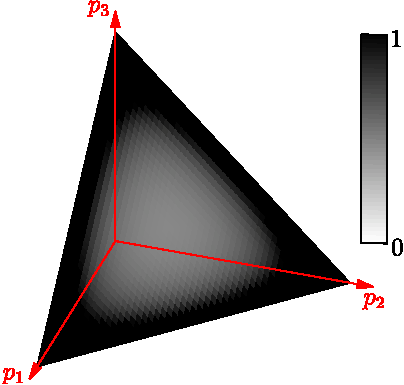
\includegraphics[width=0.3\textwidth]{figures/dirichletSparse.pdf}
\end{center}
\item By drawing \(\bm{\theta}^{(d)}\) and \(\bm{\phi}^{(t)}\) from a
Dirichlet distribution with small parameters \(\alpha\) and
\(\beta\) we ensure that most components are very small
with a few large components
\item To generate a document we choose a topic for each word and a
word for each topic
\item We use the categorical distribution
\begin{itemize}
\item if \(\bm{p}\) is a vector of non-negative values that sum to 1 then
\(\mathrm{Cat}(i|\bm{p}) = p_{i}\)
\item That is if \(I\sim\mathrm{Cat}(\bm{p})\) then \(I\) will be an integer, \(i\)
with probability \(p_{i}\)
\end{itemize}
\item Thus for word \(i\) of document \(d\) we first choose a topic
\(\tau_{i}^{(d)}\sim \mathrm{Cat}(\bm{\theta}^{d})\) and then we
choose a word \(w_{i}^{(d)} \sim
       \mathrm{Cat}(\bm{\phi}^{\tau_{i}^{(d)}})\)
\begin{itemize}
\item It is a slightly crazy model in that words are randomly
chosen from the topics of the document with no ordering
\end{itemize}
\item We could represent this by a rather ugly graphical model (see
Figure \ref{fig:ldagm})
\begin{figure}[htbp]
\centering
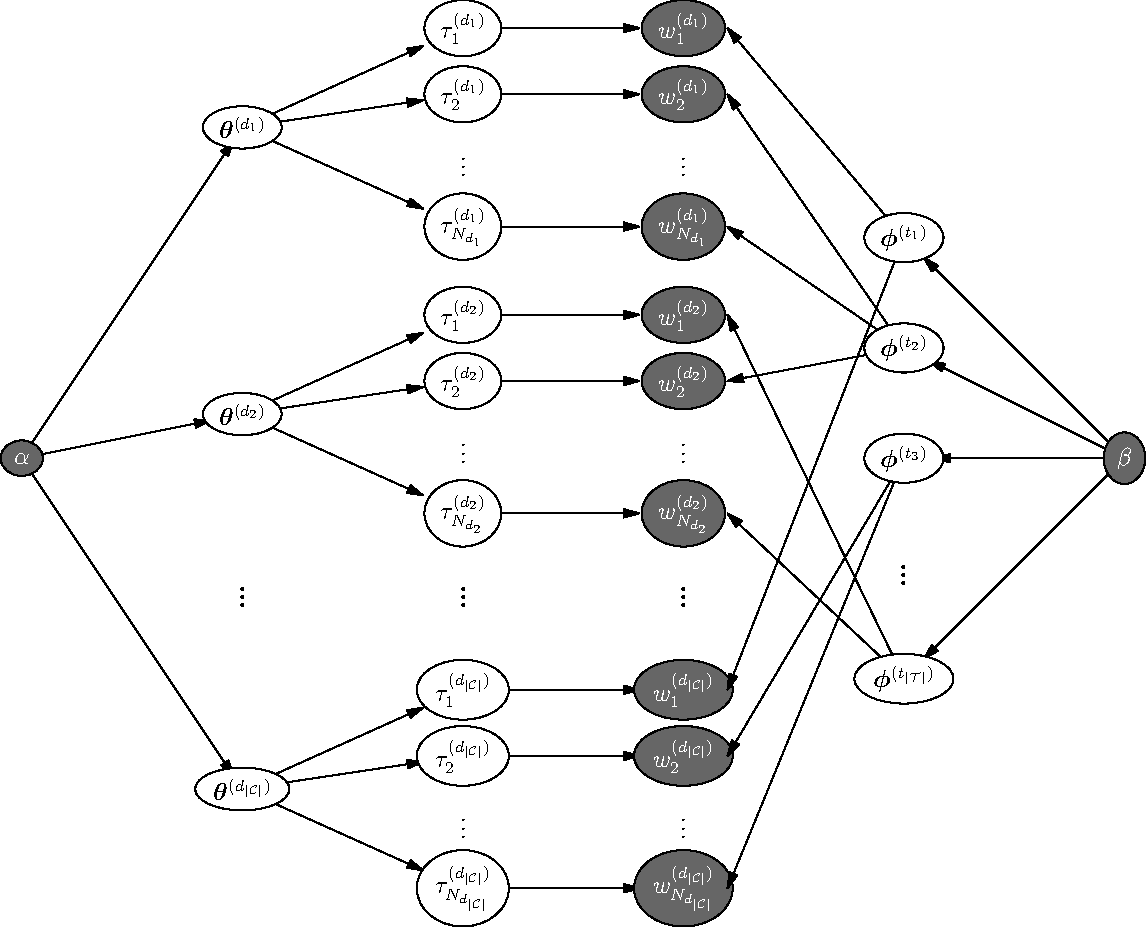
\includegraphics[width=0.6\textwidth]{../lectures/figures/LDAGM.pdf}
\caption{Graphical Model for Latent Dirichlet Allocation \label{fig:ldagm}}
\end{figure}
\item To make graphical models more manageable people have invented a
graphical means of showing repeats
\item For example, to illustrate that we have a probability vector
\(\bm{\theta}^{(d)}\) drawn from a Dirichlet distribution with
parameter \(\alpha\) for each document \(d\) in our corpus
\(\mathcal{C}\) we can use a \textbf{plate diagram}
\begin{center}
\includegraphics[width=0.3\textwidth]{../lectures/figures/GMplateSimple.pdf}
\end{center}
\item Using a plate diagram we can represent the LDA as shown in
Figure \ref{fig:ldaplate}
\begin{figure}[htbp]
\centering
\includegraphics[width=0.6\textwidth]{../lectures/figures/GMplateLDA.pdf}
\caption{Graphical Model for Latent Dirichlet Allocation \label{fig:ldaplate}}
\end{figure}
\item It takes a bit of time to decode this
\begin{itemize}
\item We have a probability vector \(\bm{\theta}^{(d)}\) for every document in our corpus
\begin{itemize}
\item this tells us the distribution of topics in the document
\item \(\bm{\theta}^{(d)}\) is drawn from a Dirichlet distribution
with parameters \(\bm{\alpha}=(\alpha,\alpha,\alpha,\ldots,\alpha)\)
\end{itemize}
\item We have a probability \(\bm{\phi}^{(\tau)}\) for every topic
\begin{itemize}
\item this tells us the distribution of words associated with a topic
\item \(\bm{\phi}^{(\tau)}\) is drawn from a Dirichlet distribution
with parameters \(\bm{\beta} = (\beta,\beta,\beta,\ldots,\beta)\)
\end{itemize}
\item For each document, \(d\), and each word, \(w_{i}^{(d)}\) in the document we have
\begin{itemize}
\item a topic \(\tau^{(d)}_{i}\) drawn from \(\bm{\theta}^{(d)}\)
\item the words \(w_{i}^{(d)}\) are drawn from \(\bm{\phi}^{(\tau^{(d)}_{i})}\)
\item that is it depends both on the topic \(\tau^{(d)}_{i}\) and
on the distributions of words associated with that topic
\end{itemize}
\item In practice I am usually given the documents with words (the
words are observed)
\item I have shaded what is usually taken to be observed (for
\(\alpha\) and \(\beta\) we usually just choose these from the
start---we could learn then so they would not be observed)
\end{itemize}
\item The graphical model helps us write down the joint distribution
\item We define matrices to denote all the variables
\begin{align*}
 \bm{W} &= (\bm{w}^{(d)} | d\in\mathcal{C})\quad \text{with} \quad
 \bm{w}^{(d)}=(w_1^{(d)},\, w_2^{(d)},\, \ldots,\, w_{N_d}^{(d)}),
 \quad \text{and}\quad w_i^{(d)} \in \mathcal{V} \\
  \bm{T} &= (\tau^{(d)}_i | d\in\mathcal{C}\;\wedge\;
   i\in\{1,\,2,\,\ldots, N_d\})\quad \text{with} \quad \tau^{(d)}_i \in
   \mathcal{T} \\
  \bm{\Theta} &=(\bm{\theta}^{(d)} | d\in\mathcal{C})\quad \text{with}
   \quad \bm{\theta}^{(d)} = (\theta^{(d)}_t | t \in \mathcal{T})\in
  \Lambda^{|\mathcal{T}|} \\
  \bm{\Phi} &= (\bm{\phi}^{(t)} | t \in \mathcal{T}) \quad \text{with}
 \quad \bm{\phi}^{(t)} = (\phi^{(t)}_w | w \in \mathcal{V}) \in
 \Lambda^{|\mathcal{V}|}
\end{align*}
\item Then the joint distribution is given by
\begin{align*}
\hspace{-1cm}        \Prob{\bm{W},\bm{T},\bm{\Theta},\bm{\Phi}\big|\alpha,\beta} =
 & \left(\prod_{t\in\mathcal{T}} \Dist[Dir]{\bm{\phi}^{(t)}\big|\beta\bm{1}}\right)
  \Biggl(\prod_{d\in\mathcal{C}} \Dist[Dir]{\bm{\theta}^{(d)}\big|\alpha\bm{1}}
  \prod_{i=1}^{N_d} \Dist[Cat]{\tau_i^{(d)}\big| \bm{\theta}^{(d)}}
  \Dist[Cat]{w_i^{(d)} \big| \bm{\phi}^{(\tau_i^{(d)})}}\Biggr)
  \end{align*}
\item It is now a technical exercise to compute the quantities of interest
\item For example \(f(\bm{\Theta},\bm{\Phi}|\bm{W},\alpha,\beta)\) will
tell us about the words associated with the topics that are
present in the corpus and the topics associated with each document
\item Note that we would marginalise out \(\bm{T}\)
\item There are different techniques for computing these
probabilities, e.g. using MCMC or variational approximations
\end{itemize}
\end{itemize}



\section{Exercise}
\label{sec:org74214ff}

\subsection{Cakes \label{sec:exCakes}}
\label{sec:org0e8413b}
\begin{itemize}
\item Write a program to compute the probability of various events
concerning cakes
\item To compute all the probabilities (sometimes inefficiently) we can
sum over all values our variables can take
\item I have done this somewhat inefficiently in the answers
\end{itemize}


\section{Answers}
\label{sec:org09856f9}

\subsection{Cakes}
\label{sec:org40caeea}
\begin{itemize}
\item I am using asymptote which I usually use for drawing diagrams,
but its a language with C syntax
\item Port this to a language of your choice
\end{itemize}

\begin{minted}[]{c}
real pcGab(int a, int b, int c) { // P(C|A,B)
  real p;
  if (a==1 && b==1)
    p = 1;
  else if (a==1 || b==1)
    p = 0.95;
  else
    p = 0.05;
  if (c==1)
    return p;
  else
    return 1-p;
}

real pa(int a) { // P(A)
  return (a==1)? 0.2:0.8;
}

real pb(int b) { // P(B)
  return (b==1)? 0.1:0.9;
}

real pd(int d, int c) { // P(D|C)
  real p = (c==1)? 0.8:0.1;
  return (d==1)? p:1-p;
}

real pe(int e, int c) {// P(E|C)
  real p = (c==1)? 0.6:0;
  return (e==1)? p:1-p;
}



typedef real func(int, int, int, int, int); // define signature of general function

real expect(func f) { // compute expectations exhaustively
  real sum = 0;
  for (int a=0; a<=1; ++a) {
    for (int b=0; b<=1; ++b) {
      for (int c=0; c<=1; ++c) {
	for (int d=0; d<=1; ++d) {
	  for (int e=0; e<=1; ++e) {
	    sum += f(a,b,c,d,e)*pcGab(a,b,c)*pa(a)*pb(b)*pd(d,c)*pe(e,c);
	  }
	}

      }
    }
  }
  return sum;
}

/* Define functions to find expectations */
/* These are all indicator funtions so I end up with probabilities */

real f(int a, int b, int c, int d, int e) {return 1;}
real fa(int a, int b, int c, int d, int e) {return a;}
real fb(int a, int b, int c, int d, int e) {return b;}
real fab(int a, int b, int c, int d, int e) {return a*b;}
real fc(int a, int b, int c, int d, int e) {return c;}
real fac(int a, int b, int c, int d, int e) {return a*c;}
real fbc(int a, int b, int c, int d, int e) {return b*c;}
real fabc(int a, int b, int c, int d, int e) {return a*b*c;}
real fd(int a, int b, int c, int d, int e) {return d;}
real fe(int a, int b, int c, int d, int e) {return e;}
real fde(int a, int b, int c, int d, int e) {return d*e;}
real fcd(int a, int b, int c, int d, int e) {return c*d;}
real fce(int a, int b, int c, int d, int e) {return c*e;}

real fcde(int a, int b, int c, int d, int e) {return c*d*e;}


write("Check joint probability is normalised: ", expect(f));
write("P(A=1) = ", expect(fa));
write("P(B=1) = ", expect(fb));
write("P(A=1)*P(B=1) = ", expect(fa)*expect(fb));
write("P(A=1,B=1) = ", expect(fab));
write("Note P(A=1,B=1) = P(A=1)*P(B=1)");
write("-");

real Pc = expect(fc);
write("P(C=1) = ", Pc);
real PaGc = expect(fac)/Pc;
real PbGc = expect(fbc)/Pc;
real PabGc = expect(fabc)/Pc;
write("P(A=1|C=1) = ", PaGc);
write("P(B=1|C=1) = ", PbGc);
write("P(A=1|C=1)*P(B=1|C=1) = ", PaGc*PbGc);
write("P(A=1,B=1|C=1) = ", PabGc);
write("Note: P(A=1,B=1|C=1) != P(A=1|C=1)*P(B=1|C=1)");
write("-");

write("P(D=1) = ", expect(fd));
write("P(E=1) = ", expect(fe));
write("P(D=1)*P(E=1) = ", expect(fd)*expect(fe));
write("P(D=1,E=1) = ", expect(fde));
write("Note: P(D=1,E=1) != P(D=1)*P(E=1)");
write("-");

write("P(D=1|C=1) = ", expect(fcd)/Pc);
write("P(E=|C=11) = ", expect(fce)/Pc);
write("P(D=1|C=1)*P(E=1|C=1) = ", expect(fcd)/Pc*expect(fce)/Pc);
write("P(D=1,E=1|C=1) = ", expect(fcde)/Pc);
write("Note: P(D=1,E=1|C=1) = P(D=1|C=1)*P(E=1|C=1)");
\end{minted}

\subsection{Result from program}
\label{sec:org6feda02}
\begin{verbatim}
Check joint probability is normalised: 1
P(A=1) = 0.2
P(B=1) = 0.1
P(A=1)*P(B=1) = 0.02
P(A=1,B=1) = 0.02
Note P(A=1,B=1) = P(A=1)*P(B=1)
-
P(C=1) = 0.303
P(A=1|C=1) = 0.63036303630363
P(B=1|C=1) = 0.316831683168317
P(A=1|C=1)*P(B=1|C=1) = 0.19971898179917
P(A=1,B=1|C=1) = 0.066006600660066
Note: P(A=1,B=1|C=1) != P(A=1|C=1)*P(B=1|C=1)
-
P(D=1) = 0.3121
P(E=1) = 0.1818
P(D=1)*P(E=1) = 0.05673978
P(D=1,E=1) = 0.14544
Note: P(D=1,E=1) != P(D=1)*P(E=1)
-
P(D=1|C=1) = 0.8
P(E=|C=11) = 0.6
P(D=1|C=1)*P(E=1|C=1) = 0.48
P(D=1,E=1|C=1) = 0.48
Note: P(D=1,E=1|C=1) = P(D=1|C=1)*P(E=1|C=1)
\end{verbatim}
\end{document}
